\chapter*{Liste af Riter}\addcontentsline{toc}{chapter}{Liste af Riter}
\begin{rite*}[Bevægelse]
    \centering
    \includegraphics[width=\textwidth]{mainstuff/riteBilleder/Bevægelse.png}
\Large \textbf{Navn:} Bevægelse\\
\textbf{Rite:} Kin\\
\textbf{Bevægelse:} Hånden knyttes og føres væk fra brystet.\\
\end{rite*}

\begin{rite*}[Dæmon]
    \centering
    \includegraphics[width=\textwidth]{mainstuff/riteBilleder/Dæmon.png}
\Large \textbf{Navn:} Dæmon\\
\textbf{Rite:} Daemon\\
\textbf{Bevægelse:} Fingrene holdes i den klassiske ”hil-satan” stilling og føres en gang op mod ansigtet og en gang ned mod navlen.
\end{rite*}

\begin{rite*}[Død]
    \centering
    \includegraphics[width=\textwidth]{mainstuff/riteBilleder/Død.png}
\Large \textbf{Navn:} Død\\
\textbf{Rite:} Morbis\\
\textbf{Bevægelse:} En flad hånd føres i en halvcirkel foran brystet.
\end{rite*}

\begin{rite*}[Give]
    \centering
    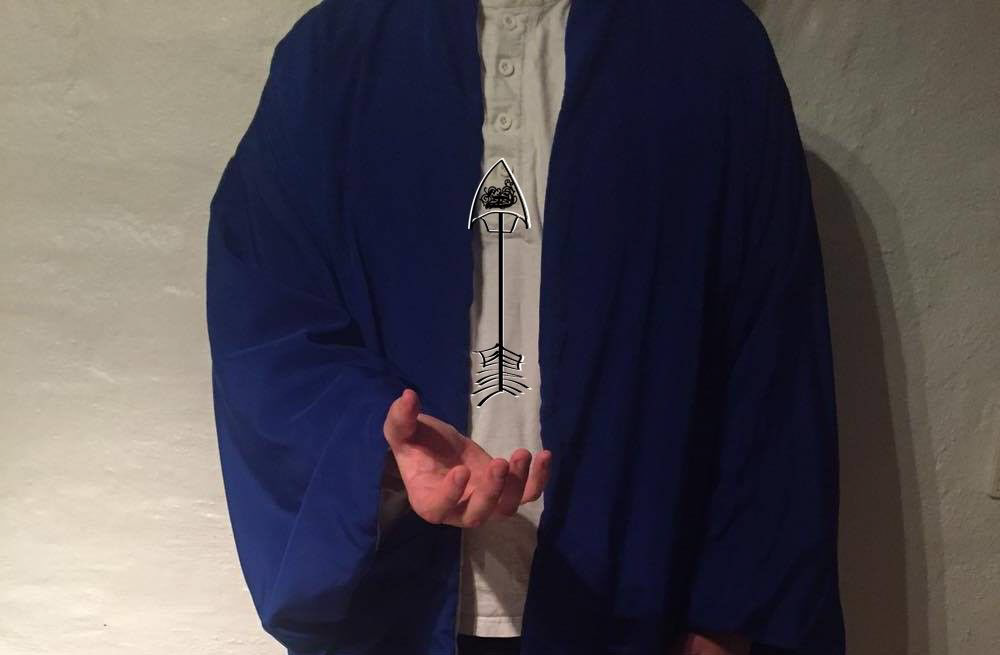
\includegraphics[width=\textwidth]{mainstuff/riteBilleder/Give.png}
\Large \textbf{Navn:} Give\\
\textbf{Rite:} Presentis\\
\textbf{Bevægelse:} Hånden formes som en skål og føres fra navlen mod ansigtet.
\end{rite*}

\begin{rite*}[Ild]
    \centering
    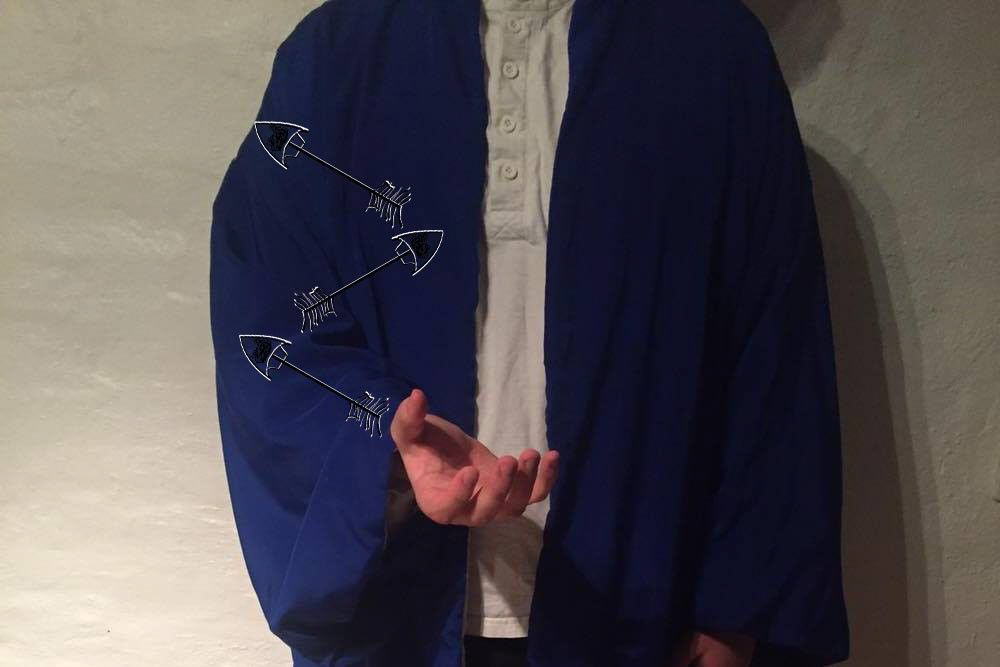
\includegraphics[width=\textwidth]{mainstuff/riteBilleder/Ild.png}
\Large \textbf{Navn:} Ild\\
\textbf{Rite:} Pyros\\
\textbf{Bevægelse:} Hånden formes som en skål og føres fra navlen op mod ansigtet i et glidende zigzag mønster.
\end{rite*}

\begin{rite*}[Jord]
    \centering
    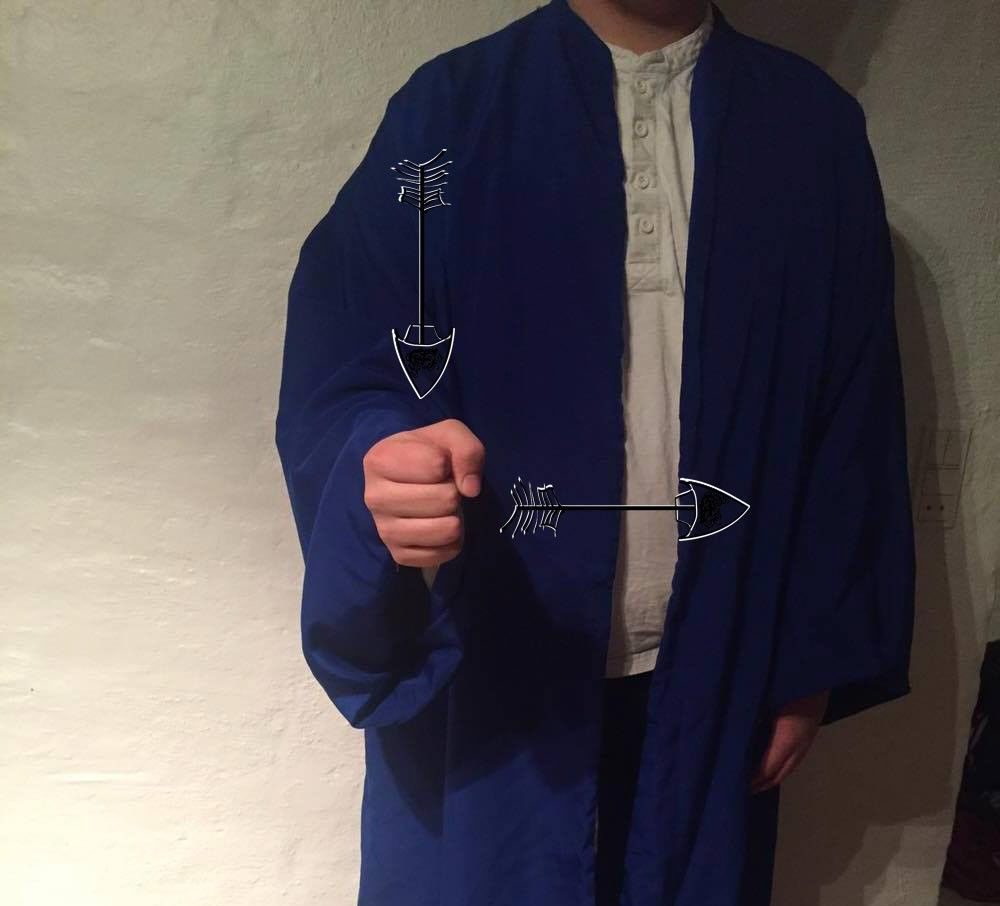
\includegraphics[width=\textwidth]{mainstuff/riteBilleder/Jord.png}
\Large \textbf{Navn:} Jord\\
\textbf{Rite:} Terra\\
\textbf{Bevægelse:} Hånden knyttes og føres fra ansigtet til navlen og derefter til venstre.
\end{rite*}

\begin{rite*}[Liv]
    \centering
    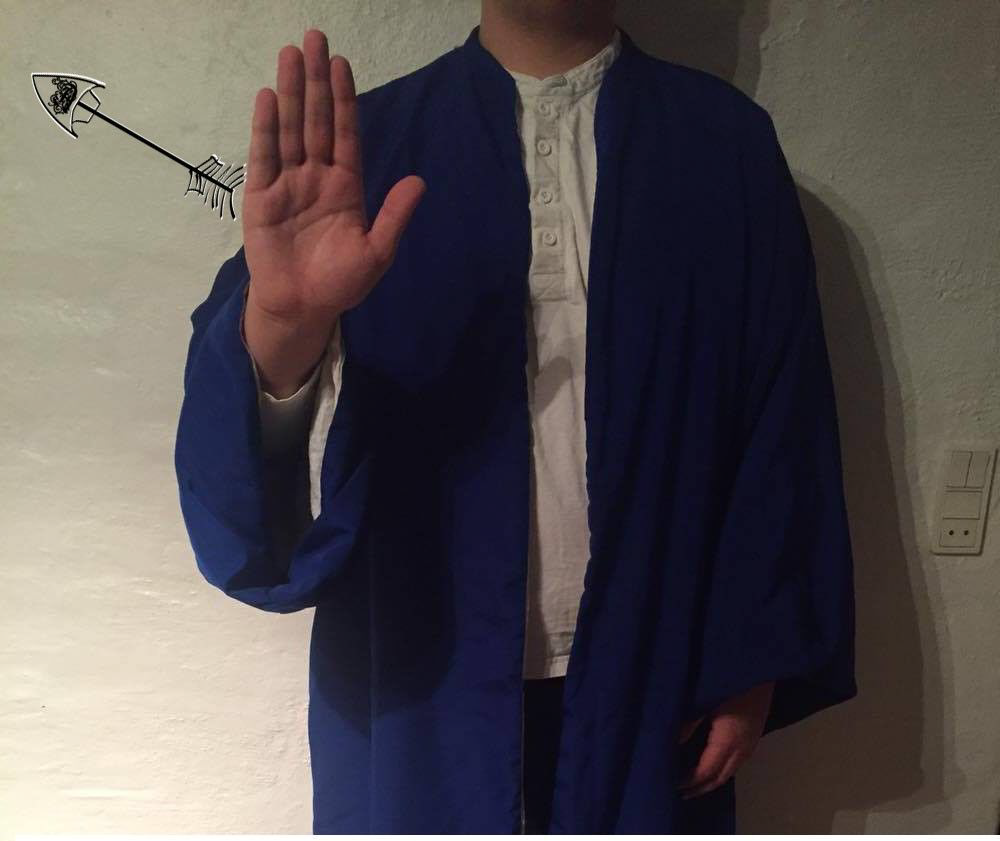
\includegraphics[width=\textwidth]{mainstuff/riteBilleder/Liv.png}
\Large \textbf{Navn:} Liv\\
\textbf{Rite:} Vita\\
\textbf{Bevægelse:} En flad hold holdes ud foran dit bryst som et klassisk stoptegn.
\end{rite*}

\begin{rite*}[Magi]
    \centering
    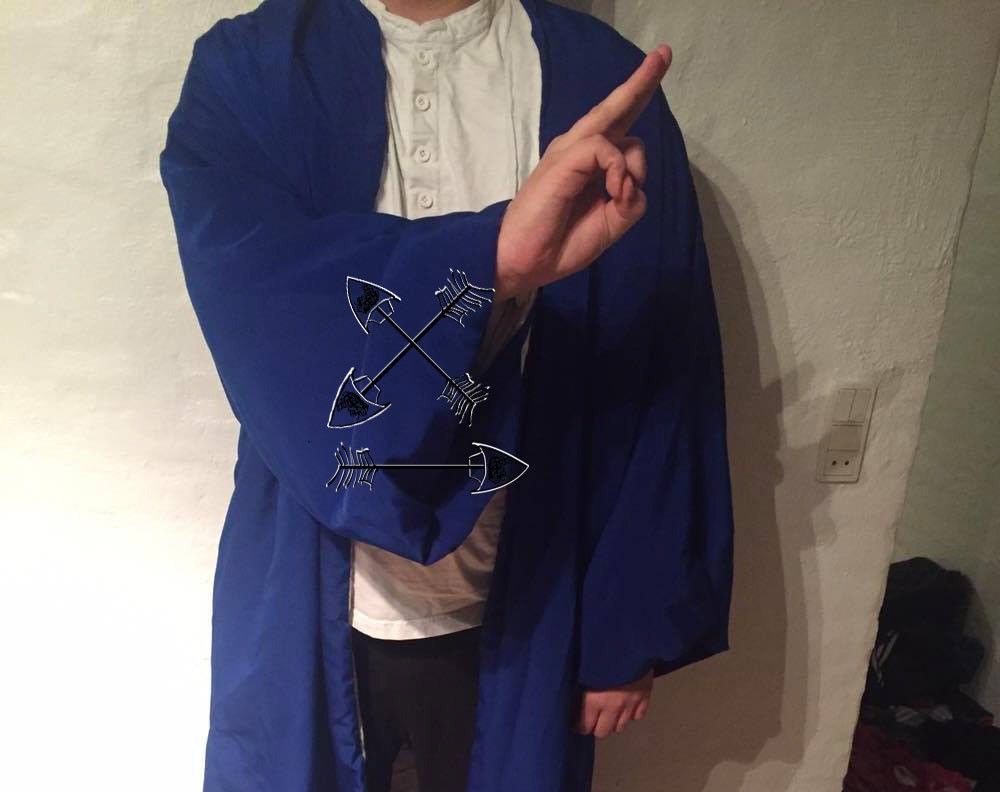
\includegraphics[width=\textwidth]{mainstuff/riteBilleder/Magi.png}
\Large \textbf{Navn:} Magi\\
\textbf{Rite:} Magus\\
\textbf{Bevægelse:} Ringefingeren og langefingeren på hånden rettes ud og resten knyttes ind mod håndfladen. Hånden føres fra venstre skulder mod højre hofte derefter mod venstre hofte og så mod højre skulder
\end{rite*}

\begin{rite*}[Tanke]
    \centering
    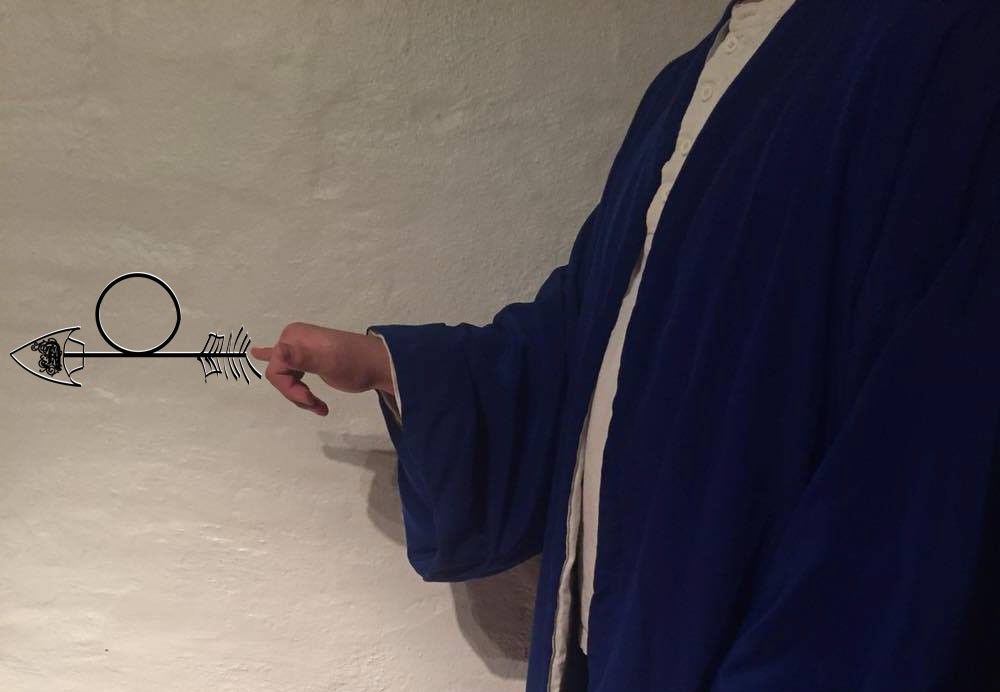
\includegraphics[width=\textwidth]{mainstuff/riteBilleder/Tanke.png}
\Large \textbf{Navn:} Tanke\\
\textbf{Rite:} Mentalis\\
\textbf{Bevægelse:} Tommelfinger og lillefinger strækkes ud mens resten knyttes. Hånden føres i en jævn bevægelse ind imod kroppen og derefter væk fra kroppen.
\end{rite*}

\begin{rite*}[Trække]
    \centering
    \includegraphics[width=\textwidth]{mainstuff/riteBilleder/Trække.png}
\Large \textbf{Navn:} Trække\\
\textbf{Rite:} Tran\\
\textbf{Bevægelse:} Hånden formes som en skål og føres fra brystet mod navlen.
\end{rite*}

\begin{rite*}[Vand]
    \centering
    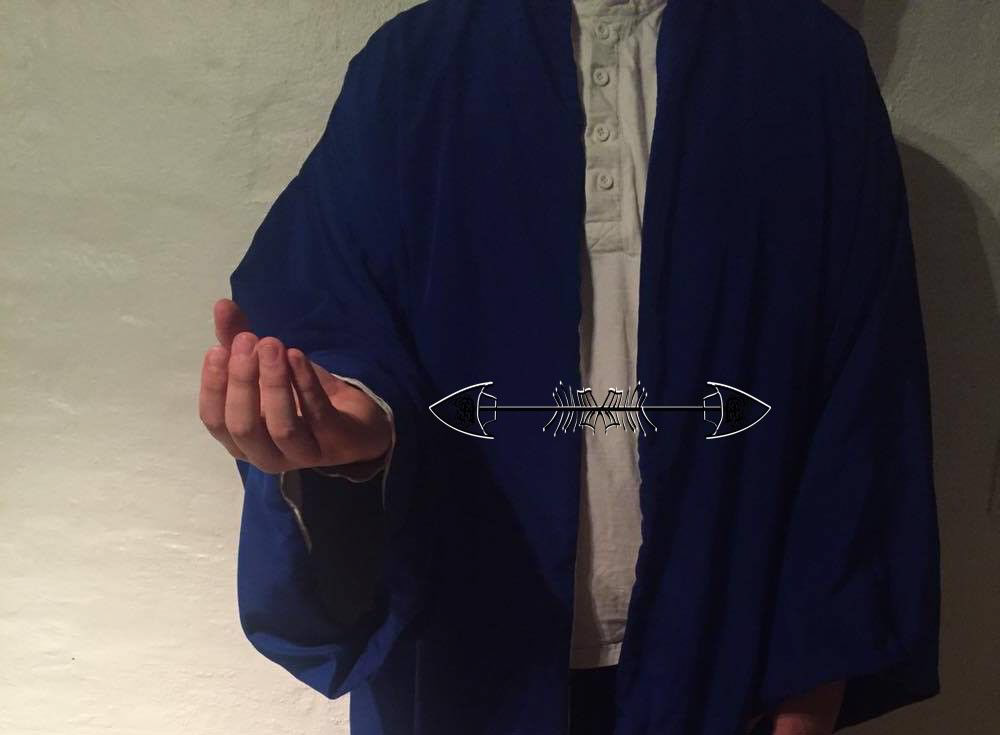
\includegraphics[width=\textwidth]{mainstuff/riteBilleder/Vand.png}
\Large \textbf{Navn:} Vand\\
\textbf{Rite:} Aqua\\
\textbf{Bevægelse:} Hånden formes således at den ser ud til at holde om en usynlig bold. Denne stilling føres nu først til højre og derefter til venstre
\end{rite*}